
%%% use twocolumn and 10pt options with the asme2ej format
\documentclass[twocolumn,10pt]{asme2ej}

\usepackage{epsfig} %% for loading postscript figures
\usepackage{listings}
\usepackage{amsmath}
\usepackage{graphicx}
\usepackage{grffile}
\usepackage{pdfpages}
\usepackage{algpseudocode}
\usepackage{courier}
\usepackage{tikz}
\newcommand*\circled[1]{\tikz[baseline=(char.base)]{
            \node[shape=circle,draw,inner sep=2pt] (char) {#1};}}
%\usepackage{multicol}


% Custom colors
\usepackage{color}
\usepackage{listings}
\usepackage{framed}
\usepackage{caption}
\usepackage{bm}
\captionsetup[lstlisting]{font={small,tt}}

\definecolor{mygreen}{rgb}{0,0.6,0}
\definecolor{mygray}{rgb}{0.5,0.5,0.5}
\definecolor{mymauve}{rgb}{0.58,0,0.82}

\lstset{ %
  backgroundcolor=\color{white},   % choose the background color; you must add \usepackage{color} or \usepackage{xcolor}
  basicstyle=\ttfamily\footnotesize, % the size of the fonts that are used for the code
  breakatwhitespace=false,         % sets if automatic breaks should only happen at whitespace
  % breaklines=true,                 % sets automatic line breaking
  captionpos=b,                    % sets the caption-position to bottom
  commentstyle=\color{mygreen},    % comment style
  deletekeywords={...},            % if you want to delete keywords from the given language
  escapeinside={\%*}{*)},          % if you want to add LaTeX within your code
  extendedchars=true,              % lets you use non-ASCII characters; for 8-bits encodings only, does not work with UTF-8
  frame=single,                    % adds a frame around the code
  keepspaces=true,                 % keeps spaces in text, useful for keeping indentation of code (possibly needs columns=flexible)
  columns=flexible,
  keywordstyle=\color{blue},       % keyword style
  language=Python,                 % the language of the code
  morekeywords={*,...},            % if you want to add more keywords to the set
  numbers=left,                    % where to put the line-numbers; possible values are (none, left, right)
  numbersep=5pt,                   % how far the line-numbers are from the code
  numberstyle=\tiny\color{mygray}, % the style that is used for the line-numbers
  rulecolor=\color{black},         % if not set, the frame-color may be changed on line-breaks within not-black text (e.g. comments (green here))
  showspaces=false,                % show spaces everywhere adding particular underscores; it overrides 'showstringspaces'
  showstringspaces=false,          % underline spaces within strings only
  showtabs=false,                  % show tabs within strings adding particular underscores
  stepnumber=1,                    % the step between two line-numbers. If it's 1, each line will be numbered
  stringstyle=\color{mymauve},     % string literal style
  tabsize=4,                       % sets default tabsize to 2 spaces
}



%% The class has several options
%  onecolumn/twocolumn - format for one or two columns per page
%  10pt/11pt/12pt - use 10, 11, or 12 point font
%  oneside/twoside - format for oneside/twosided printing
%  final/draft - format for final/draft copy
%  cleanfoot - take out copyright info in footer leave page number
%  cleanhead - take out the conference banner on the title page
%  titlepage/notitlepage - put in titlepage or leave out titlepage
%
%% The default is oneside, onecolumn, 10pt, final

\title{MAE 267 -- Project 4\\Parallel, Multi-Block, Finite-Volume Methods\\For Solving 2D Heat Conduction}

%%% first author
\author{Logan Halstrom
    \affiliation{
	PhD Graduate Student Researcher\\
	Center for Human/Robot/Vehicle Integration and Performance\\
	Department of Mechanical and Aerospace Engineering\\
	University of California, Davis\\
	Davis, California 95616\\
    Email: ldhalstrom@ucdavis.edu
    }
}

\begin{document}
\maketitle

%%%%%%%%%%%%%%%%%%%%%%%%%%%%%%%%%%%%%%%%%%%%%%%%%%%%%%%%%%%%%%%%%%%%%%
\section{Statement of Problem}

This analysis details the solution of the steady-state temperature distribution on a 1m x 1m block of steel with Dirichlet boundary conditions (Eqn~\ref{dirichlet}).  Single-processor solutions were previously performed on a square, non-uniform grids rotatated in the positive z-direction by $rot=30^o$.  Two grids of 101x101 points and 501x501 points were used to solve the equation of heat transfer.  Temperature was uniformly initialized to a value of 3.5 and the solution was iterated until the maximum residual found was less than $1.0x10^{-5}$.  The equation for heat conduction (Eqn~\ref{heat}) was solved using an explicit, node-centered, finite-volume scheme, with an alternative distributive scheme for the second-derivative operator.  Steady-state temperature distribution was saved in a PLOT3D unformatted file, and CPU wall time of the solver was recorded.

Now, the code has been modified to decompose the domain into sub-domains refered to as blocks.  Boundary and neighbor information for each block is stored so that connectivity can be accurately assessed when communication between blocks is required.  The block domain, associated meshes, and initial temperature distribution are initialized and then saved to restart files.  These are read in at the beginning of the solver.

%%%%%%%%%%%%%%%%%%%%%%%%%%%%%%%%%%%%%%%%%%%%%%%%%%%%%%%%%%%%%%%%%%%%%%%%
\section{Equations and Algorithms}

The solver developed for this analysis utilizes a finite-volume numerical solution method to solve the transient heat conduction equation (Eqn~\ref{heat}).

\begin{equation}
\begin{split}
\rho c_p \frac{\partial T}{\partial t} =
    k \left[ \frac{\partial^2 T}{\partial x^2}
    + \frac{\partial^2 T}{\partial y^2} \right]
\end{split}
\label{heat}
\end{equation}

\noindent The solution is initialized with the Dirichlet boundary conditions (Eqn~\ref{dirichlet}).

\begin{equation}
\begin{split}
T = &\left\{ \begin{array}{lll}
    \mbox{$5.0 \left[ \sin\left( \pi x_p \right) + 1.0 \right]$} & \mbox{for } &j = j_{max} \\
    \mbox{$\left| \cos\left( \pi x_p \right)\right|+1.0$} & \mbox{for } &j = 0 \\
    \mbox{$3.0 y_p + 2.0$} & \mbox{for } &i = 0, \, i_{max}
     \end{array} \right.
\end{split}
\label{dirichlet}
\end{equation}

\noindent Grids were generated according to the following (Eqn~\ref{grideqn})

\begin{equation}
\begin{split}
   rot &= 30.0 \frac{\pi}{180.0} \\
   x_p &= \cos \left[ 0.5\pi \frac{i_{max}-i}{i_{max}-1} \right] \\
   y_p &= \cos \left[ 0.5\pi \frac{j_{max}-j}{j_{max}-1} \right] \\
x(i,j) &= x_p \cos(rot) + (1.0 - y_p) \sin(rot) \\
y(i,j) &= y_p \cos(rot) + x_p \sin(rot)
\end{split}
\label{grideqn}
\end{equation}

\noindent To solve Eqn~\ref{heat} numerically, the equation is discretized according to a node-centered finite-volume scheme, where first-derivatives at the nodes are found using Green's theorem integrating around the secondary control volumes.  Trapezoidal, counter-clockwise integration for the first-derivative in the x-direction is achieved with Eqn~\ref{FVx1st}.

\begin{equation}
\begin{split}
\frac{\partial T}{\partial x} = \frac{1}{2Vol_{i+\frac{1}{2},j+\frac{1}{2}}}
    \left[ \left(T_{i+1,j} + T_{i+1,j+1} \right)Ayi_{i+1,j} \right. \\
    \left. - \left(T_{i,j} + T_{i,j+1} \right)Ayi_{i,j} \right. \\
    \left. - \left(T_{i,j+1} + T_{i+1,j+1} \right)Ayi_{i,j+1} \right. \\
    \left. - \left(T_{i,j} + T_{i+1,j} \right)Ayi_{i,j} \right]
\end{split}
\label{FVx1st}
\end{equation}

\noindent A similar scheme is used to find the first-derivative in the y-direction.

Size of each block (no ghost nodes)
Total mesh points in I-direction including block overlap points:

\begin{equation}
\begin{split}
IMAX_{tot} = IMAX + (N-1)
\end{split}
\label{overlappoints}
\end{equation}

Points in I-direction per block

\begin{equation}
\begin{split}
IMAXBLK = \frac{IMAX_{tot}}{N} = \frac{IMAX + (N-1)}{N} = 1 + \frac{IMAX-1}{N}
\end{split}
\label{pointsperblock}
\end{equation}

For points in J-direction, replace I with J and N with M

Global starting index of each block in I-direction:

\begin{equation}
\begin{split}
IMIN_{block} = IMIN_{global} + (IMAXBLK-1)(I-1)
\end{split}
\label{blockstartingindex}
\end{equation}

\noindent where I counts blocks in the direction of N and $IMIN_{global}=1$.  The first block in the N-direction has a global starting index of 0, and IMAXBLK must be reduced by one to account for the single-point overlap at block boundaries.

%%%%%%%%%%%%%%%%%%%%%%%%%%%%%%%%%%%%%%%%%%%%%%%%%%%%%%%%%%%%%%%%%%%%%%

% %%\vspace{-2em}
% \begin{figure}[htb]
% \begin{center}
% \includegraphics[width=0.5\textwidth]{../Results/finalMulti/501_10x10.png}
% \caption{Steady-state temperature solution for 501x501 grid decomposed into 10x10 blocks}
% \label{501x10x10}
% \end{center}
% \end{figure}
% %%\vspace{-2em}

% %%\vspace{-2em}
% \begin{figure}[htb]
% \begin{center}
% 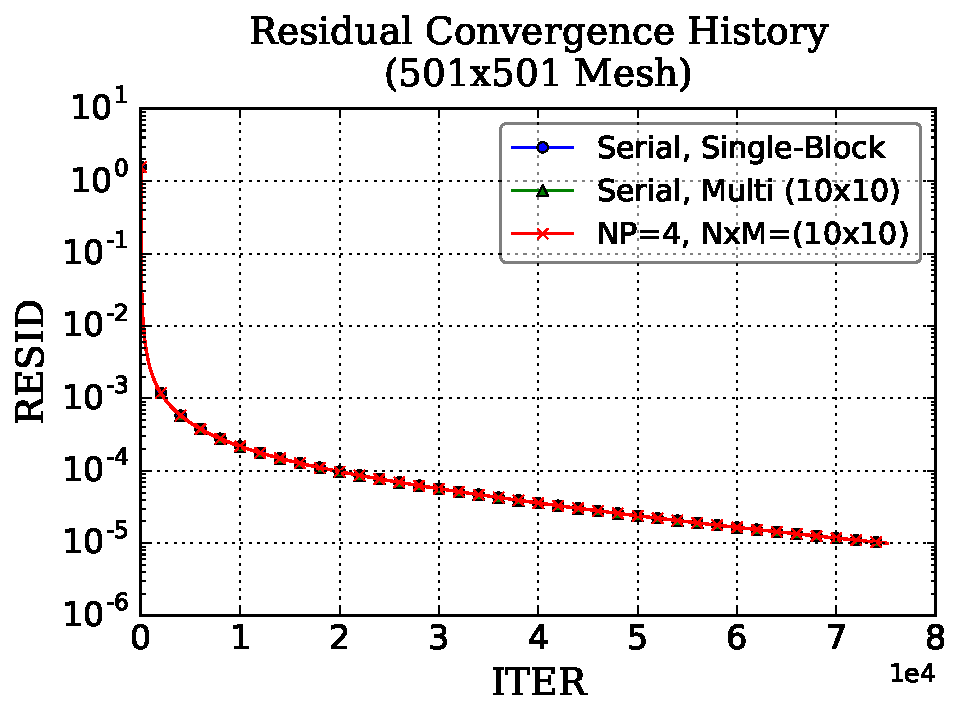
\includegraphics[width=0.5\textwidth]{../Results/ResHist.png}
% \caption{Residual history for solving a 501x501 grid with a single block solver and a 10x10 multi-block solver}
% \label{reshist}
% \end{center}
% \end{figure}
% %%\vspace{-2em}

\section{Results and Discussion}

All simulations in this analysis were run on a 501x501 point grid, once with a single block solver and once with at 10x10 multi-block solver.  Fig~\ref{501x10x10} portrays the multi-block solution, which is comparable to that of the single block solver.  Convergence histories of the two solvers are compared in Fig~\ref{reshist}.  It can be seen that the two solvers are comparable in performance, both following a similar convergence path and converging at almost the same iteration.

Actual solver times are compared in Appendix A.  The multi-block solver was found to be approximately 11 seconds (2.6\%) faster than the single block solver.  This may be due to more code streamlining in the later project.  It can be expected that the speed of the multi-block solver will improve even further when linked-lists are employed to navigate neighbor boundary actions (this capability is currently functional in the code, but does not work on HPC1, so a logic-based approach was used for this project.)





%%%%%%%%%%%%%%%%%%%%%%%%%%%%%%%%%%%%%%%%%%%%%%%%%%%%%%%%%%%%%%%%%%%%%%%%
\section{Conclusion}

Decomposing the domain introduced unforseen complications in adapting the single block solver.  In some cases, it was as simple as adding a third loop for the block number, but in others (especially in updating the ghost nodes) considerable thought and error-checking was required.  This implies that adapting the code for parallel processing will be an equally complicated step, so it is beneficial that we are adapting our codes modularly in stages.

%%%%%%%%%%%%%%%%%%%%%%%%%%%%%%%%%%%%%%%%%%%%%%%%%%%%%%%%%%%%%%%%%%%%%%%%
% \section{References}
% \begin{description}
% \item[] 1. Bogard, D.G., Teiderman, W.G. ``Burst detection with single-point velocity measurements'', \emph{Journal of Fluid Mechanics}, 162:389-413, 1986.
% \end{description}








%%%%%%%%%%%%%%%%%%%%%%%%%%%%%%%%%%%%%%%%%%%%%%%%%%%%%%%%%%%%%%%
% \clearpage
\onecolumn
\appendix       %%% starting appendix

\section*{Appendix A: Solver Performace Comparison} \label{times}
% \lstinputlisting[caption=Single block solver performance, language={}]{../Results/finalSingle/SolnInfo.dat}
% \lstinputlisting[caption=Multi block solver performance, language={}]{../Results/finalMulti/SolnInfo.dat}

\section*{Appendix B: Multi-Block Grid Decomposition Code}
\lstinputlisting[caption=Grids are decomposed into blocks and information pertaining to neighbors is stored using the GRIDMOD module, language=Fortran]{../modules.f90}

\section*{Appendix C: Multi-Block Solver Subroutines}
\lstinputlisting[caption=Main subroutines used for solving heat transfer on a multi-block grid, language=Fortran]{../subroutines.f90}

\clearpage

\section*{Appendix D: Multi-Block Plot3D Reader-Writer}
\lstinputlisting[caption=Code for saving formatted multiblock PLOT3D solution files and reading restart files, language=Fortran]{../inout.f90}

% \clearpage
\section*{Appendix E: Other Relevant Codes}
\lstinputlisting[caption=Wrapper program, language=Fortran]{../main.f90}



%%%%%%%%%%%%%%%%%%%%%%%%%%%%%%%%%%%%%%%%%%%%%%%%%%%%%%%%%%%%%%%%%%%%%%
%\clearpage


%%%%%%%%%%%%%%%%%%%%%%%%%%%%%%%%%%%%%%%%%%%%%%%%%%%%%%%%%%%%%%%%%%%%%%
% The bibliography is stored in an external database file
% in the BibTeX format (file_name.bib).  The bibliography is
% created by the following command and it will appear in this
% position in the document. You may, of course, create your
% own bibliography by using thebibliography environment as in
%
% \begin{thebibliography}{12}
% ...
% \bibitem{itemreference} D. E. Knudsen.
% {\em 1966 World Bnus Almanac.}
% {Permafrost Press, Novosibirsk.}
% ...
% \end{thebibliography}

% Here's where you specify the bibliography style file.
% The full file name for the bibliography style file
% used for an ASME paper is asmems4.bst.
%\bibliographystyle{asmems4}

% Here's where you specify the bibliography database file.
% The full file name of the bibliography database for this
% article is asme2e.bib. The name for your database is up
% to you.
%\bibliography{asme2e}

%%%%%%%%%%%%%%%%%%%%%%%%%%%%%%%%%%%%%%%%%%%%%%%%%%%%%%%%%%%%%%%%%%%%%%


\end{document}
